\documentclass{article}
\usepackage{graphicx} % new way of doing eps files
\usepackage{listings} % nice code layout
\usepackage[usenames]{color} % color
\definecolor{listinggray}{gray}{0.9}
\definecolor{graphgray}{gray}{0.7}
\definecolor{ans}{rgb}{1,0,0}
\definecolor{blue}{rgb}{0,0,1}
% \Verilog{title}{label}{file}
\newcommand{\Verilog}[3]{
  \lstset{language=Verilog}
  \lstset{backgroundcolor=\color{listinggray},rulecolor=\color{blue}}
  \lstset{linewidth=\textwidth}
  \lstset{commentstyle=\textit, stringstyle=\upshape,showspaces=false}
  \lstset{frame=tb}
  \lstinputlisting[caption={#1},label={#2}]{#3}
}


\author{your names}
\title{Lab title}

\begin{document}
\maketitle

\section{Introduction}
Introduction with problem overview, your design procedure, and rationale.  Be as brief as possible to let me know the big picture of the lab.

\section{Interface}
This section should identify the inputs and outputs of each stage.  To do this, rather than explaining them in paragraph form, please take the datapath diagram in Figure ~\ref{fig:datapath} and add your signal names to the diagram.  This will give you a graphical representation of your system that can be quickly evaluated to determine the meaning of each signal.  For any additional signals that appear on your simulation results, put the signals in a table with a short description of that signal.

\begin{figure}
	\caption{Full Non-Pipelined Datapath}\label{fig:datapath}
	\begin{center}
		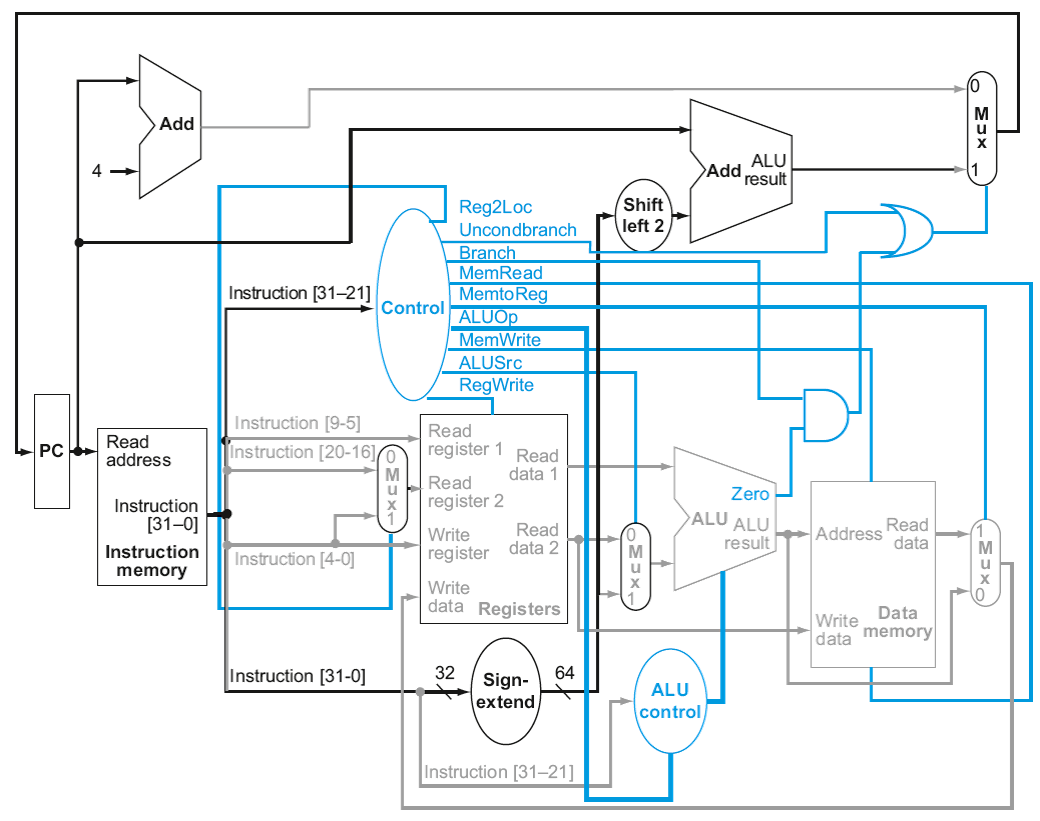
\includegraphics[width=\textwidth]{../images/non_pipelined_datapath.png}
	\end{center}
\end{figure}

\section{Design}
Most of the design for the datapath is pre-determined by Figure ~\ref{fig:datapath}.  The item that is not pre-determined is the timing.  For this Design section, you do not need to add any substantial text.  Please just reference a timing diagram that shows the timing between each stage.  See Figure ~\ref{fig:timing_diagram_example} for an example of a simple timing diagram.

\begin{figure}
	\caption{Timing Diagram Example}\label{fig:timing_diagram_example}
	\begin{center}
		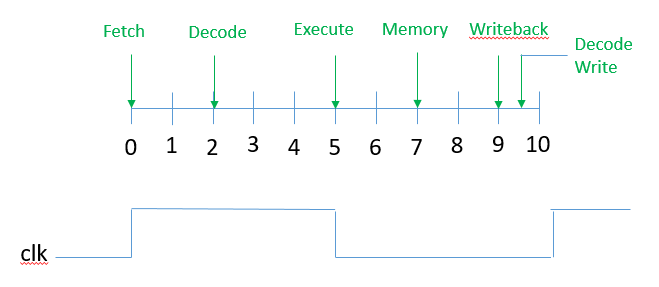
\includegraphics[width=\textwidth]{../images/timing_diagram_example.png}
	\end{center}
\end{figure}

\section{Implementation}
The Verilog code and explanations of why you implemented this way.  Code should be included in the report like Listing~\ref{code:reg} on page~\pageref{code:reg}.  For this lab, you should describe iMemory and iWriteback (and any submodules you feel are necessary).

\Verilog{Verilog code for implementing a register.}{code:reg}{../code/1_fetch/register.v}

\section{Test}
This is where you discuss the test cases you wrote, and what they were designed to test.  You should discuss expected errors as well as random errors.  Please include:
\begin{enumerate}
	\item Testbench code (in this case, datapath.v because it is the top-level module)
	\item List of assembly commands that you have been using to test your datapath since the iDecode stage
	\item Binary for the commands you have been using to test your datapath since the iDecode stage
	\item Expected Results Table
	\item Simulation Results from these commands (that should match your expected results).  A sample simulation diagram is in Figure~\ref{fig:regtest} on page~\pageref{fig:regtest}.
	\item Assembly code for the "Division Problem" C code that I gave you
	\item Instruction Data File for the Division Problem
	\item Register Data File for the Division Problem
	\item Memory Data File for the Division Problem
	\item Simulation Results for the Division Problem
\end{enumerate}

\Verilog{Verilog code for testing a register.}{code:regtest}{../code/1_fetch/register_test.v}

\begin{figure}
\begin{center}
\caption{Timing diagram for the register test.}\label{fig:regtest}
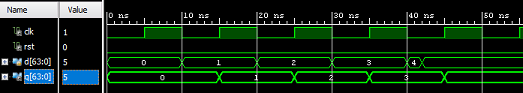
\includegraphics[width=0.9\textwidth]{../images/registertiming.png}
\end{center}
\end{figure}

\section{Conclusions}
Overview the main points you want to stick in peoples minds and answer key questions you want to stick in peoples minds.  Did it work?  How well? What would you have done differently?  What did you learn?
\end{document} 